\documentclass[12pt]{article}

\usepackage[a4paper,  top=1.3in, bottom=1.4in, left=1.4in, right=1.5in]{geometry}

\usepackage[utf8]{inputenc}
\usepackage[T1]{fontenc}
\usepackage{amsmath}
\usepackage{amsfonts}
\usepackage{amssymb}


\usepackage{graphicx, float}
\usepackage{adjustbox}
\graphicspath{{images/}}

% \renewcommand{\figurename}{Slika}



\renewcommand{\baselinestretch}{1.2} % Line spacing

% Parskip and parindent
\setlength{\parindent}{0pt} % Begin of paragraph indentation
\setlength{\parskip}{1em} % Paragraph spacing

%--- for references ---------
\usepackage[
    backend=biber,
    style=numeric,
    sorting=none
    ]{biblatex}

\addbibresource{bibliography.bib}
\AtBeginBibliography{\vspace*{10pt}}
%----------------------------

%----------- toc ------------------------
\usepackage{tocloft}
\usepackage{fancyhdr}
% \setlength{\cftbeforesecskip}{0pt} % Adjust the spacing before section entries
% \setlength{\cftbeforesubsecskip}{0pt} % Adjust the spacing before subsection entries
%----------------------------------------

\begin{document}

% Title Page
\newgeometry{top=1in, bottom=1in, left=1in, right=1in} % New margins for title page
\begin{titlepage}
    \begin{center}
        
        % add your university logo here
        % negative value moves the logo up
        \vspace*{-1in}
        
\includegraphics[width=0.4\textwidth]{raf_logo.png}

        % set font size to 14pt
        \vspace{1in}
        \Large
        \textbf{Review on the topic of}
        
        % set horizontal margin for the title to 1.5in and center it
        \vspace{1in}
        \Huge
        \textbf{Retrieval-Augmented Generation (RAG)}
        
        \vspace{1in}


            \fontsize{18pt}{18pt}\selectfont
            \textbf{Course: Data mining} \\
            \vspace*{1.5in}
            
            \begin{center}
            \normalsize
            \begin{tabular}{p{0.75\textwidth} p{0.5\textwidth}}
                \fontsize{14pt}{18pt}\selectfont   
                \textbf{Advisor:} & 
            
                \fontsize{14pt}{18pt}\selectfont
                \textbf{Student:} \\
                prof. Nemanja Ilić & Vanja Kovinić \\
            \end{tabular}
            \end{center}

            \vspace*{\fill}

            \normalsize
            Belgrade, January 2025.


            
        \end{center}
    \end{titlepage}
    \restoregeometry % Restore original margins

    \newpage
    \newgeometry{top=1.3in, bottom=2.2in, left=1.4in, right=1.4in} % New margins for title page
    
    % Table of Contents
    \renewcommand{\contentsname}{Contents}
    \addtocontents{toc}{\protect\thispagestyle{empty}}
    \tableofcontents
    \thispagestyle{empty} % Remove page numbers

    \restoregeometry % Restore original margins
    \newpage
    \pagenumbering{arabic}
    \setcounter{page}{1}

    \section{Introduction}
    Recent advances in \textbf{Large Language Models (LLMs)} have revolutionized natural language 
    processing, demonstrating remarkable capabilities in tasks ranging from text generation 
    to complex reasoning. Models like \textbf{GPT-4} \cite{gpt4technicalreport} and 
    \textbf{LLaMA} \cite{llama3} have achieved good performance in understanding and generating 
    human-like text. However, these models face significant limitations that impact their practical 
    deployment and reliability in real-world applications.
    
    One of the fundamental challenges with traditional LLMs is their reliance on static 
    knowledge encoded in model parameters during training. This approach presents several 
    critical issues. 
    \begin{itemize}
        \item First, the knowledge contained within these models becomes outdated as 
        new information emerges, requiring costly and time-consuming retraining or fine-tuning 
        processes.
        
        \item Second, the models are constrained by their parameter count, with even the 
        largest models unable to capture all potentially relevant information.
        
        \item Third, fine-tuning these models on new data can lead to forgetting, 
        where the model loses previously acquired knowledge while adapting to new information. 
    \end{itemize}
    
    To address these limitations, researchers have developed \\ \textbf{Retrieval-Augmented Generation (RAG)} \cite{rag_paper}, 
    a novel architecture that combines the generative capabilities of LLMs with dynamic access 
    to external knowledge sources. RAG represents a paradigm shift in how we approach 
    language models, moving from purely parametric knowledge to a hybrid system that can 
    actively retrieve and incorporate relevant information during inference.
    
    The core innovation of RAG lies in its ability to decompose the knowledge acquisition 
    and generation processes. Instead of relying solely on information encoded in model 
    parameters, RAG systems maintain a separate knowledge base that can be easily updated 
    without modifying the underlying language model. This separation provides several 
    advantages: it allows for real-time knowledge updates, reduces the memory requirements 
    for storing information, and maintains consistent access to accurate, verifiable information.
    
    \section{Large Language Models: Background and Limitations}
    
    \subsection{Understanding Language Models}
    LLMs are probabilistic systems trained to predict the next token 
    in a sequence based on the provided context. During training, these models process vast 
    amounts of text data, learning to capture patterns, relationships, and factual information 
    within their parameters. The knowledge acquired during training is encoded in billions of 
    parameters - for instance, \textbf{GPT-3} \cite{gpt3} contains 175 billion parameters, while models 
    like \textbf{LLaMA 2} \cite{llama2} can range from 7 billion to 70 billion parameters.

    The training process involves exposing the model to a diverse corpus of text data, 
    allowing it to learn language patterns and accumulate knowledge about various topics. 
    This knowledge, however, is static and bounded by the training cutoff date, creating 
    what is known as the knowledge cutoff problem. Any information or events occurring after 
    the training period are unknown to the model, regardless of their significance.

    \subsection{Limitations of Traditional LLMs}
    
    \subsubsection{The Knowledge Cutoff Problem}
    
    The knowledge cutoff represents a fundamental limitation of LLMs. For example, a model 
    trained with data up to 2022 would have no inherent knowledge of significant events or 
    technological developments that occurred in 2023. This limitation becomes increasingly 
    problematic as time passes, making the model's knowledge progressively outdated.
    
    \subsubsection{Fine-tuning Challenges}
    
    Organizations facing the knowledge cutoff problem might consider fine-tuning as a solution. 
    However, fine-tuning presents several significant challenges:

    \begin{itemize}
        \item \textbf{Cost Implications:} Fine-tuning large models requires substantial 
        computational resources and expertise, making it prohibitively expensive for many organizations.

        \item \textbf{Parameter Limitations:} The number of parameters in a model may not be 
        sufficient to capture all desired knowledge. Even large models like \textbf{LLaMA 2} (70B) 
        have finite capacity for storing information.

        \item \textbf{Forgetting:} Fine-tuning can lead to the model forgetting previously learned 
        information. For instance, a model heavily fine-tuned on recent events might lose its ability
        to reason about historical contexts.
    \end{itemize}

    \subsection{Prompt Engineering as a Partial Solution}
    Prompt engineering has emerged as a technique to mitigate the knowledge cutoff problem by 
    providing relevant context within the input prompt. This approach allows users to "teach" 
    the model new information on the fly, enabling it to reason about and generate responses 
    based on up-to-date information (\textit{Figure 1}).

    \subsubsection{Benefits of Prompt Engineering}
    \begin{itemize}
    \item \textbf{Dynamic Knowledge Integration:} Users can provide current information without 
    modifying the model's parameters.
    \item \textbf{Flexibility:} The context can be tailored to specific queries or use cases.
    \item \textbf{Verifiability:} Since the context is explicitly provided, the source of 
    information is transparent and can be verified.
    \end{itemize}

    \begin{figure}[h!]
        \centering
        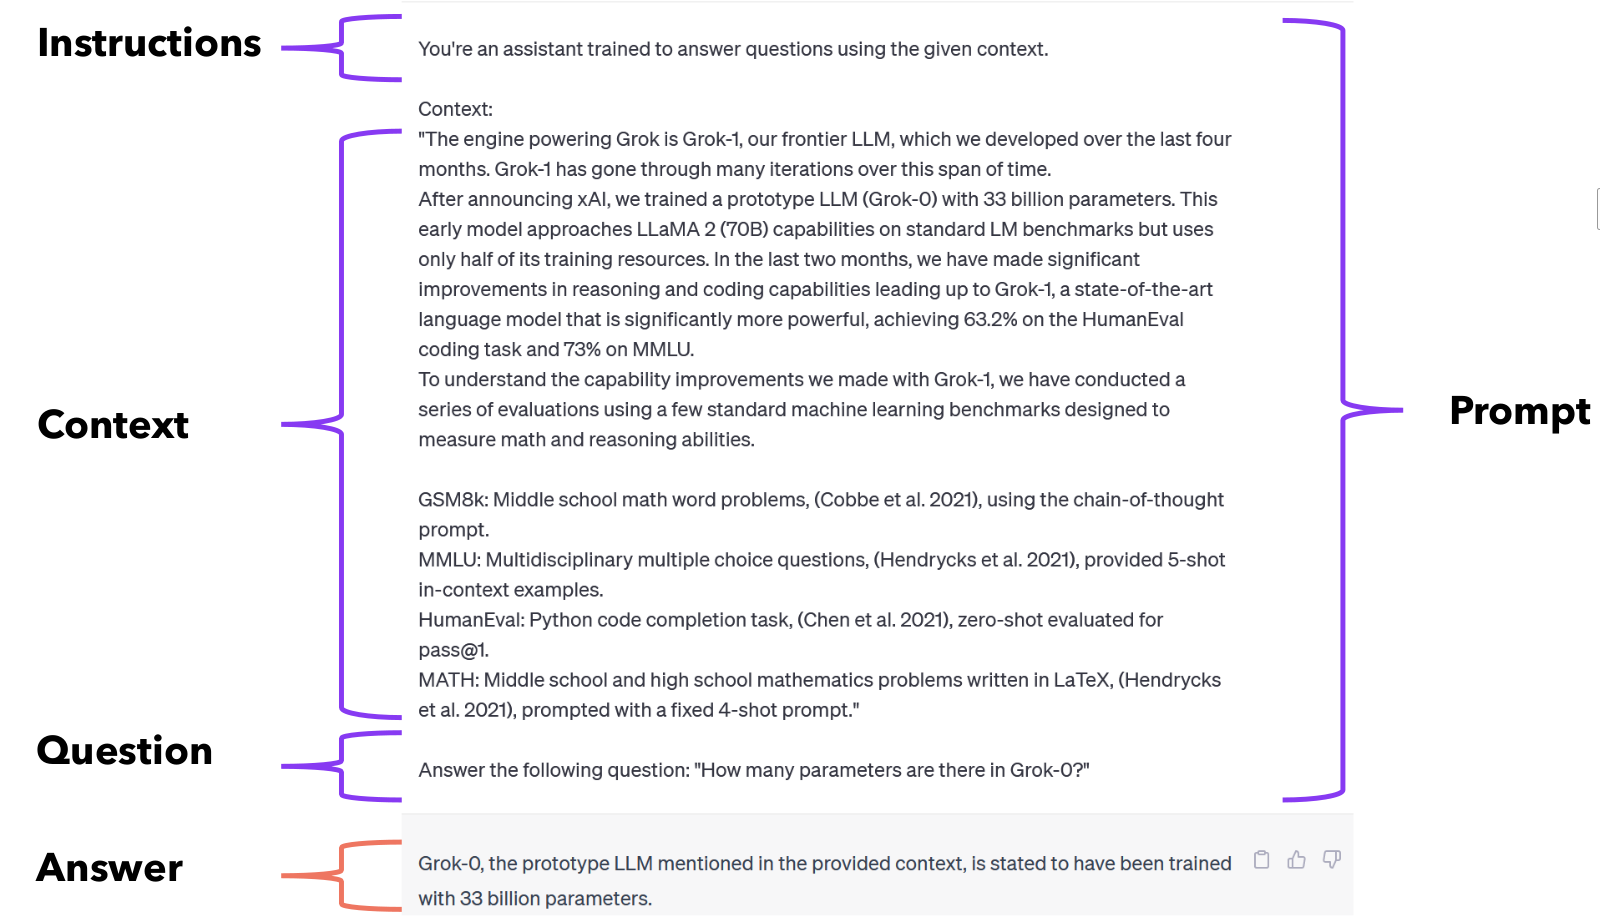
\includegraphics[width=1.0\textwidth]{prompt_engineering.png}
        \caption{Example where user provides context with answer inside the prompt to enhance the LLMs response \cite{prompt_engineering}}
        \label{fig:visual_cortex}
    \end{figure}

    \subsubsection{Limitations of Prompt Engineering}
    
    However, prompt engineering comes with significant drawbacks:
    \begin{itemize}
    \item \textbf{Context Window Constraints:} Every token used for context reduces the 
    available space for the actual query and response. For example, if a model has a 4,096 
    token limit, providing 3,000 tokens of context leaves only 1,096 tokens for the query and response.
    
    \item \textbf{Manual Intervention:} Users must manually select and provide relevant context, 
    which can be time-consuming and may require expertise in the subject matter.
        
    \item \textbf{Context Selection Challenge:} Determining which context is relevant for a 
    given query can be difficult, especially for complex or ambiguous questions.    
    \end{itemize}

    \newpage
    \subsection{The Need for Alternative Approaches}
    While prompt engineering provides a workable solution for incorporating new knowledge 
    into LLM interactions, its limitations make it suboptimal for many real-world applications.
    These limitations have motivated the development of more sophisticated approaches to 
    augmenting LLM knowledge, leading to the emergence of Retrieval-Augmented Generation (RAG) 
    as a promising solution. RAG addresses many of the limitations of both traditional LLMs 
    and prompt engineering by providing a systematic way to incorporate external knowledge while 
    maintaining efficiency and scalability.


    \section{Retrieval-Augmented Generation}
    \subsection{RAG Architecture}
    Retrieval-Augmented Generation represents a significant advancement in language model architecture 
    by introducing a dynamic knowledge retrieval component into the generation process. Unlike 
    traditional LLMs that rely solely on their trained parameters, RAG systems maintain a separate 
    knowledge base that can be queried during inference.
    \newpage
    \subsubsection{Components and Their Interactions}
    The core components of a RAG system include:
    \begin{itemize}
    \item \textbf{Query Encoder:} Transforms user queries into dense vector representations
    \item \textbf{Document Index:} Stores preprocessed documents and their vector embeddings
    \item \textbf{Retrieval System:} Performs efficient similarity search to find relevant documents
    \item \textbf{Generator:} The base language model that produces the final response
    \end{itemize}
    These components work in concert, with each stage's output serving as input for the next stage in the pipeline (\textit{Figure 2}).

    \begin{figure}[h!]
        \vspace{1cm}
        \centering
        \adjustbox{scale=0.3,center}{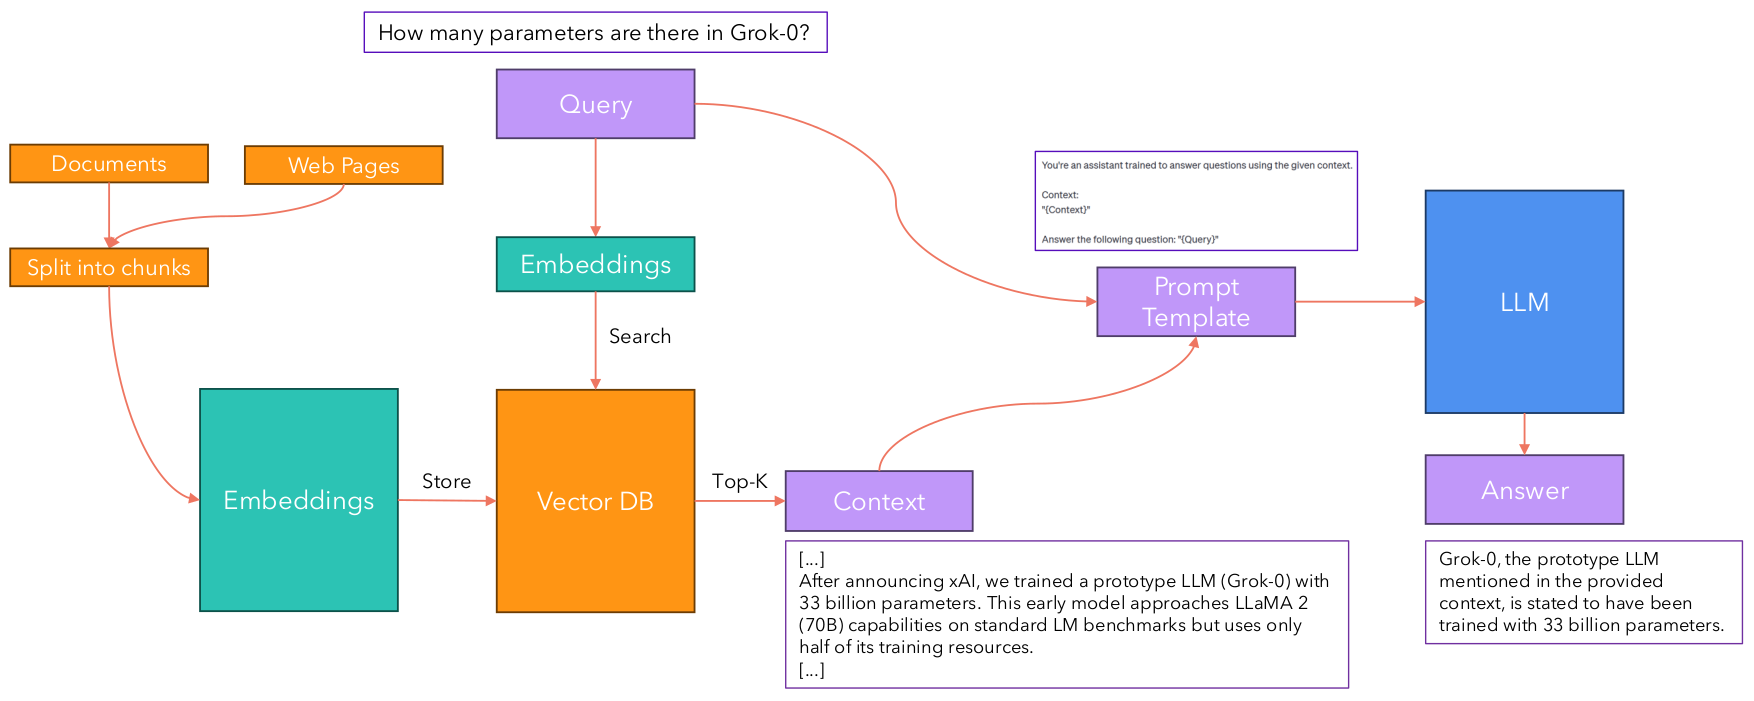
\includegraphics{rag_overview.png}}
        \caption{Overview of the RAG pipeline \cite{prompt_engineering}}
    \end{figure}

    \newpage

    \subsubsection{Query Processing}
    Query processing begins with the transformation of the user's input query into a dense vector representation. 
    This process, known as query embedding, uses the same encoding mechanism applied to documents in the knowledge 
    base, ensuring compatibility for similarity comparisons. The query encoder typically employs a pre-trained model 
    such as \textbf{Sentence-BERT} \cite{sentence_bert} to generate these embeddings (\textit{Figure 3}).

    \begin{figure}[h!]
        \vspace{1cm}
        \centering
        \adjustbox{scale=0.3,center}{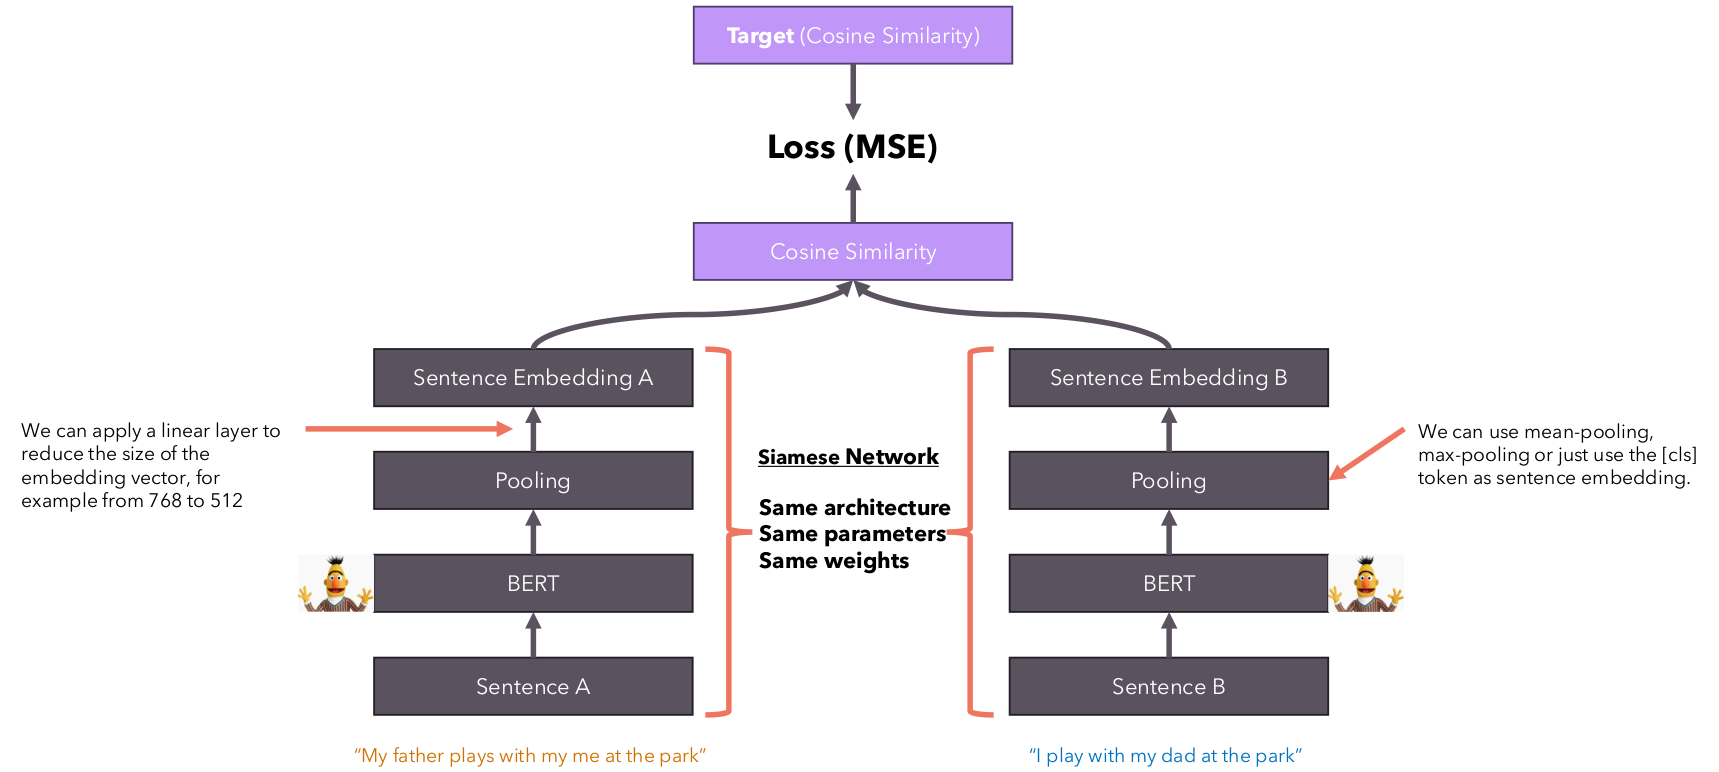
\includegraphics{sentence_bert.png}}
        \caption{Overview of the RAG pipeline \cite{prompt_engineering}}
    \end{figure}

    \subsubsection{Document Retrieval}
    The document retrieval phase involves:
    \begin{enumerate}
    \item Searching the vector database for documents with embeddings similar to the query embedding
    \item Ranking retrieved documents based on relevance scores
    \item Selecting the top-K most relevant documents to provide as context
    \end{enumerate}

    \subsubsection{Response Generation}
    The final stage combines the retrieved documents with the original query to generate a response. 
    This process typically involves:
    \begin{enumerate}
        \item Constructing a prompt that incorporates both the query and retrieved context
        \item Passing the augmented prompt to the base language model
        \item Generating a response that leverages both the model's parametric knowledge and the retrieved information
    \end{enumerate}

    \subsection{Vector Embeddings in RAG}
    \subsubsection{Purpose and Importance}
    Vector embeddings serve as the foundation of efficient information retrieval in RAG systems. 
    These dense numerical representations capture semantic meaning, allowing for
    efficient similarity comparisons between queries and documents.

    \subsubsection{Embedding Generation Techniques}
    Modern RAG systems typically employ transformer-based models for embedding generation. The process involves:
    \begin{enumerate}
    \item Tokenizing input text into subword units
    \item Passing tokens through a neural network architecture
    \item Aggregating token representations to create a single vector
    \end{enumerate}

    \newpage

    \subsubsection{Sentence-BERT Architecture}
    \textbf{Sentence-BERT (SBERT)} represents a significant advancement in embedding generation, 
    specifically optimized for sentence embeddings. Key features include:
    \begin{itemize}
    \item Siamese network architecture for comparing sentence pairs
    \item Mean pooling of token embeddings (\textit{Figure 4})
    \item Training objectives optimized for semantic similarity tasks
    \end{itemize}
    The architecture employs a "Siamese" network structure where the same BERT model processes both sentences in a pair, ensuring consistent embedding space for queries and documents.

    \begin{figure}[h!]
        \vspace{1cm}
        \centering
        \adjustbox{scale=0.3,center}{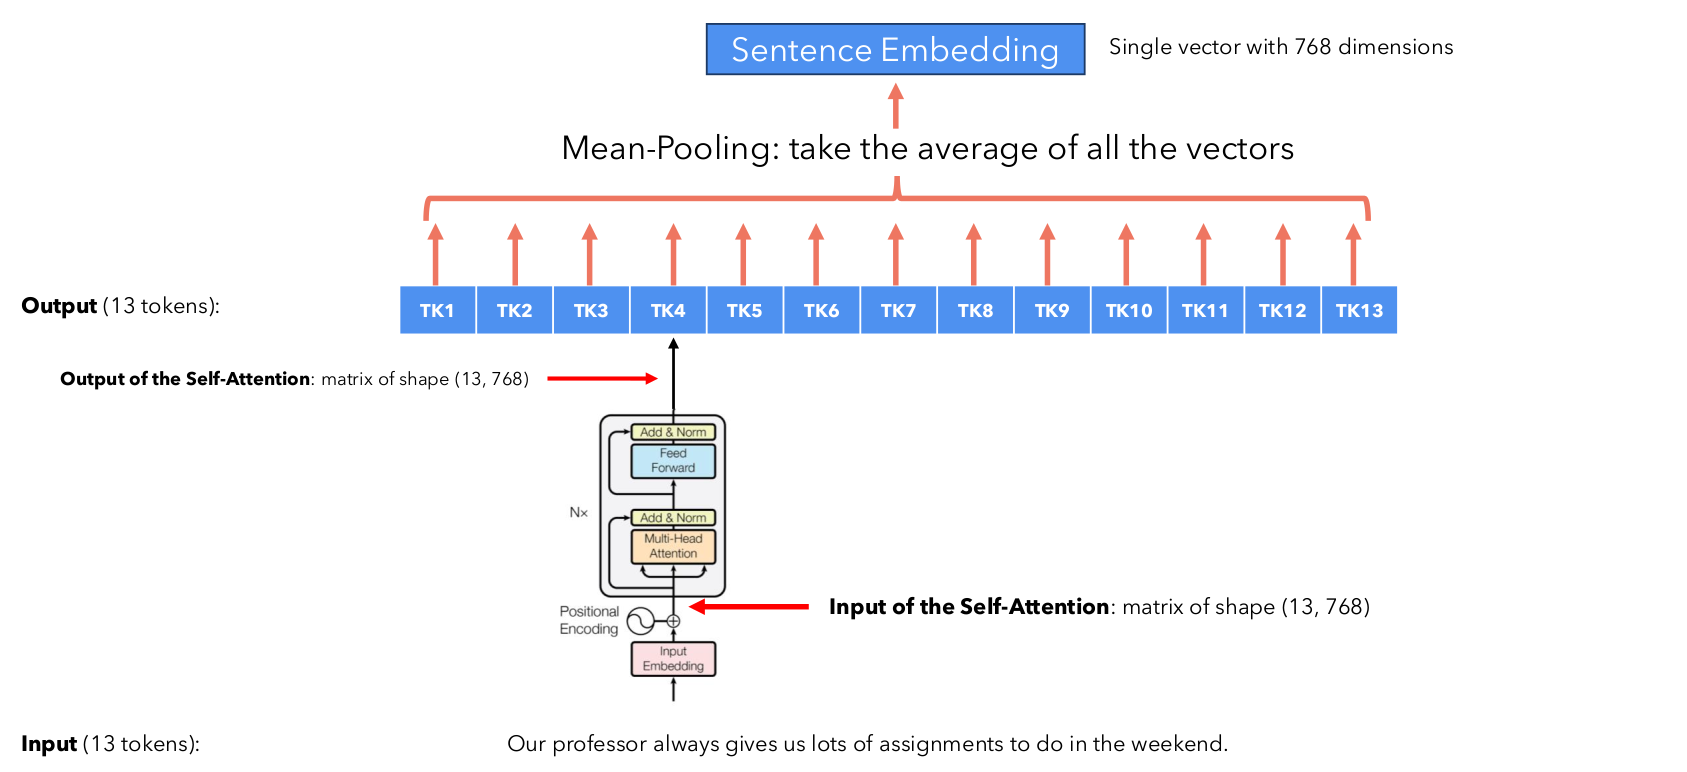
\includegraphics{sbert.png}}
        \caption{Mean pooling in Sentence BERT architecture \cite{prompt_engineering}}
    \end{figure}

    \newpage
    \subsubsection{Similarity Metrics}
    Common similarity metrics used in RAG systems include (\textit{Figure 5}):
    \begin{itemize}
    \item \textbf{Cosine Similarity:} Measures the cosine of the angle between vectors, normalized to [-1, 1]
    \item \textbf{Euclidean Distance:} Calculates the straight-line distance between vectors
    \item \textbf{Dot Product:} Computes the scalar product of two vectors
    \end{itemize}


    \begin{figure}[h!]
        \vspace{1cm}
        \centering
        \adjustbox{scale=0.5,center}{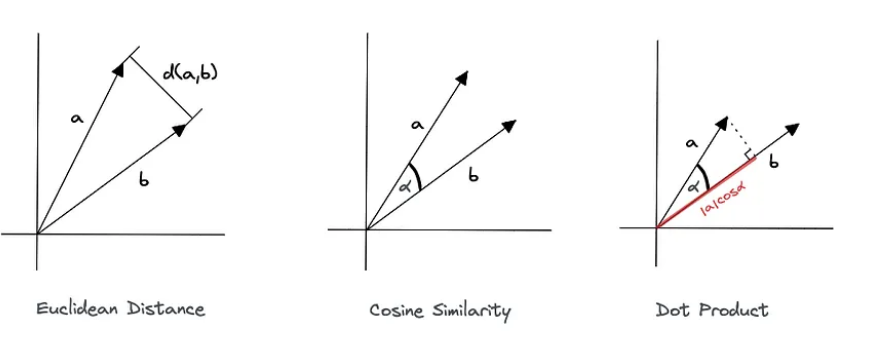
\includegraphics{rag_metrics.png}}
        \caption{Overview of different similarity metrics used in RAG databases \cite{rag_metrics}}
    \end{figure}

    \newpage
    \subsection{Vector Databases}
    \subsubsection{Role in RAG Systems}
    Vector databases serve as the backbone of efficient information retrieval in RAG systems, providing 
    fast similarity search capabilities and support for real-time updates and queries

    \subsubsection{Efficient Similarity Search}
    The challenge of similarity search in high-dimensional spaces is addressed through specialized algorithms 
    that trade perfect accuracy for significant speed improvements. This approach is particularly important 
    in RAG systems where query latency is critical.




    % \newpage
    % \printbibliography[title={References}]
\end{document}